

\tikzset{every picture/.style={line width=0.75pt}} %set default line width to 0.75pt        

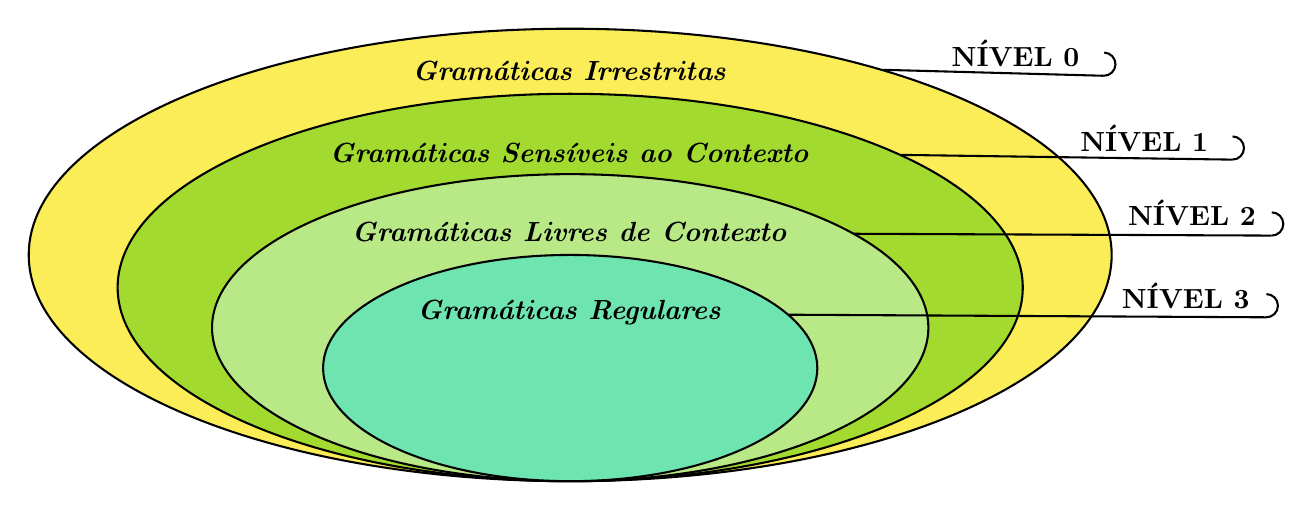
\begin{tikzpicture}[x=0.75pt,y=0.75pt,yscale=-1,xscale=1]
%uncomment if require: \path (0,478.1979217529297); %set diagram left start at 0, and has height of 478.1979217529297

%Shape: Ellipse [id:dp2589253237302658] 
\draw  [fill={rgb, 255:red, 248; green, 231; blue, 28 }  ,fill opacity=0.74 ] (8.59,137.21) .. controls (8.59,77.01) and (125.4,28.21) .. (269.48,28.21) .. controls (413.56,28.21) and (530.36,77.01) .. (530.36,137.21) .. controls (530.36,197.41) and (413.56,246.21) .. (269.48,246.21) .. controls (125.4,246.21) and (8.59,197.41) .. (8.59,137.21) -- cycle ;
%Shape: Ellipse [id:dp694350790161383] 
\draw  [fill={rgb, 255:red, 126; green, 211; blue, 33 }  ,fill opacity=0.71 ] (51.43,152.88) .. controls (51.43,101.34) and (149.05,59.56) .. (269.48,59.56) .. controls (389.91,59.56) and (487.53,101.34) .. (487.53,152.88) .. controls (487.53,204.43) and (389.91,246.21) .. (269.48,246.21) .. controls (149.05,246.21) and (51.43,204.43) .. (51.43,152.88) -- cycle ;
%Shape: Ellipse [id:dp7384199846467594] 
\draw  [fill={rgb, 255:red, 184; green, 233; blue, 134 }  ,fill opacity=1 ] (96.92,172.24) .. controls (96.92,131.39) and (174.18,98.28) .. (269.48,98.28) .. controls (364.78,98.28) and (442.04,131.39) .. (442.04,172.24) .. controls (442.04,213.09) and (364.78,246.21) .. (269.48,246.21) .. controls (174.18,246.21) and (96.92,213.09) .. (96.92,172.24) -- cycle ;
%Shape: Ellipse [id:dp08042679579621703] 
\draw  [fill={rgb, 255:red, 80; green, 227; blue, 194 }  ,fill opacity=0.7 ] (150.42,191.71) .. controls (150.42,161.61) and (203.72,137.21) .. (269.48,137.21) .. controls (335.24,137.21) and (388.54,161.61) .. (388.54,191.71) .. controls (388.54,221.81) and (335.24,246.21) .. (269.48,246.21) .. controls (203.72,246.21) and (150.42,221.81) .. (150.42,191.71) -- cycle ;
%Straight Lines [id:da6929823208677994] 
\draw    (420,48) -- (526.44,50.88) ;
\draw [shift={(526.44,50.88)}, rotate = 181.55] [color={rgb, 255:red, 0; green, 0; blue, 0 }  ][line width=0.75]      (0,0) .. controls (-3.09,0) and (-5.59,2.5) .. (-5.59,5.59) .. controls (-5.59,8.68) and (-3.09,11.18) .. (0,11.18) ;

%Straight Lines [id:da9940150469857363] 
\draw    (429,89) -- (588.44,91.28) ;
\draw [shift={(588.44,91.28)}, rotate = 180.82] [color={rgb, 255:red, 0; green, 0; blue, 0 }  ][line width=0.75]      (0,0) .. controls (-3.09,0) and (-5.59,2.5) .. (-5.59,5.59) .. controls (-5.59,8.68) and (-3.09,11.18) .. (0,11.18) ;

%Straight Lines [id:da8023852859401694] 
\draw    (406,127) -- (607.44,127.88) ;
\draw [shift={(607.44,127.88)}, rotate = 180.25] [color={rgb, 255:red, 0; green, 0; blue, 0 }  ][line width=0.75]      (0,0) .. controls (-3.09,0) and (-5.59,2.5) .. (-5.59,5.59) .. controls (-5.59,8.68) and (-3.09,11.18) .. (0,11.18) ;

%Straight Lines [id:da75358331134597] 
\draw    (375,166) -- (604.84,167.25) ;
\draw [shift={(604.84,167.25)}, rotate = 180.31] [color={rgb, 255:red, 0; green, 0; blue, 0 }  ][line width=0.75]      (0,0) .. controls (-3.09,0) and (-5.59,2.5) .. (-5.59,5.59) .. controls (-5.59,8.68) and (-3.09,11.18) .. (0,11.18) ;


% Text Node
\draw (269.48,48.76) node [scale=1] [align=left] {\textbf{\textit{Gramáticas Irrestritas}}};
% Text Node
\draw (269.48,126.28) node [scale=1] [align=left] {\textbf{\textit{Gramáticas Livres de Contexto}}};
% Text Node
\draw (269.48,88.11) node [scale=1] [align=left] {\textbf{\textit{Gramáticas Sensíveis ao Contexto}}};
% Text Node
\draw (269.48,164.97) node [scale=1] [align=left] {\textbf{\textit{Gramáticas Regulares}}};
% Text Node
\draw (484,40) node  [align=left] {\textbf{NÍVEL 0}};
% Text Node
\draw (546,81) node  [align=left] {\textbf{NÍVEL 1}};
% Text Node
\draw (569,117) node  [align=left] {\textbf{NÍVEL 2}};
% Text Node
\draw (566,157) node  [align=left] {\textbf{NÍVEL 3}};


\end{tikzpicture}
